\chapter[В каких населённых пунктах России больше рождаётся учёных, в сельских или городских?]
{В каких населённых пунктах России больше рождаётся учёных,\newline 
\hspace*{20pt}в сельских или городских?}
\label{ch:human-settlement}

В главе исследуется объект Викиданных <<\wdqName{населённый пункт}{486972}>> и его свойства. 
В~каждом из разделов представлены задачи, решённые с~помощью SPARQL-запросов. 
%
%%%%%%%%%%%%%%%% Упражнение 1 %%%%%%%%%%%%%%%% 
\marginnote{%
    \MarginQuestion
    Подсчитайте, сколько человек на~1~км\textsuperscript{2} живёт в~\ruwiki{4dNv}{Барабинске} 
и в~\ruwiki{4dNt}{Алейске}? В~каком из этих \emph{населённых пунктов} плотность населения выше?

См. ответ %~\ref{answer:human_settlements_density} 
на с.~\pageref{answer:human_settlements_density}.%
}

Был получен список населённых пунктов, 
построены пузырьковые диаграммы с~количеством населения в~<<населённых пунктах>> по странам. 
Построена диаграмма, показывающая долю населения, 
проживающего в~населённых пунктах относительно всего населения страны. 
Диаграмма показала, что высокий процент населения, проживающего в~населённых пунктах, 
приходится на сельскохозяйственные страны, в~то время как в~более индустриальных странах 
меньшая доля населения проживает в~населённых пунктах. 
%
%%%%%%%%%%%%%%%% Упражнение 2 %%%%%%%%%%%%%%%%
\marginnote{%
\MarginQuestion Герб какого отечественного или зарубежного населённого пункта изображён на рисунке?
\vspace{5pt}

    \includegraphics[width=2cm]{./chapter/human_settlement/Aznakeevskii_rayon_gerb.png}

    См. ответ %~\protect\ref{answer:flag_human_settlements} 
    на с.~\protect\pageref{answer:flag_human_settlements}.
    \label{fig:flag_question_human_settlements1}%
}

На 2017 год Википедия описывала примерно половину населённых пунктов (75 тыс.), 
Викиданные содержали менее 3\,\% таких поселений (4 тыс.) относительно данных переписи за 2010 год (155,5 тыс.). 
На 2021 год Викиданные содержат менее 12\,\% таких поселений (17 тыс.) 
относительно данных той же переписи за 2010 год. 

Для сравнения сельских и городских поселений 
построены диаграммы количества учёных, сгруппированных по родам деятельности 
и разделённых по месту рождения~--- сельское или городское.

Для поиска более полных ответов на поставленные выше задачи  
были найдены более общие классы для~объекта <<\wdqName{населённый пункт}{486972}>> 
с помощью свойства <<\wdProperty{31}{частный случай понятия}>>. 
Трудность исследования вызвана отсутствием чёткой типологии населённых пунктов 
(например, от~численности населения) в~законодательстве России и в~Викиданных.



%%%%%%%
\section{Список <<населённых пунктов>>}
%%%%%%%%%%%%%%%% Упражнение 3 %%%%%%%%%%%%%%%%
\marginnote[-\baselineskip]{%
    \MarginQuestion Это герб населённого пункта России или другой страны?
    \vspace{5pt}

    \includegraphics[width=2cm]{./chapter/human_settlement/Coat_of_Arms_of_Asbest_(Sverdlovsk_oblast).png}

    См. ответ %~\protect\ref{answer:flag_human_settlements} 
    на с.~\protect\pageref{answer:flag_human_settlements}.%
    \label{fig:flag_question_human_settlements2}%
}

Построим список всех населённых пунктов с помощью запроса~\ref{lst:human-settlement1}.

\begin{lstlisting}[ language=SPARQL, 
                    caption={\href{https://w.wiki/4d7x}{Список всех населённых пунктов}\protect\footnotemark},
                    label=lst:human-settlement1,
                    texcl 
                    ]
# List of all human settlements
SELECT ?hum ?humLabel WHERE{
  ?hum wdt:P31 wd:Q486972. # instance of human settlement
  SERVICE wikibase:label{bd:serviceParam wikibase:language "ru,en"}
}
\end{lstlisting}%
\footnotetext{Получено: \num{411393} пункта в 2017 году. SPARQL-запрос: \href{https://w.wiki/4d7x}{https://w.wiki/4d7x}.}

В 2021 году оказалось невозможным получить список населённых пунктов 
из-за большого числа объектов и поэтому слишком долгой работы запроса~\ref{lst:human-settlement1}. 
Для подсчёта числа всех населённых пунктов обратимся к функции \lstinline|COUNT()| 
в запросе~\ref{lst:human-settlement-count-classes}.

\index{SPARQL!COUNT}
\begin{lstlisting}[ language=SPARQL, 
                    caption={\href{https://w.wiki/4d7s}{Количество всех населённых пунктов}\protect\footnotemark},
                    label=lst:human-settlement-count-classes,
                    texcl 
                    ]
# Number of human settlements
SELECT (COUNT(?hum) AS ?count) WHERE {
  ?hum wdt:P31 wd:Q486972. # instance of human settlement  
}
\end{lstlisting}%
\footnotetext{Получено: \num{563126} населённых пунктов в 2021 году. SPARQL-запрос:\\\href{https://w.wiki/4d7s}{https://w.wiki/4d7s}.}

Среди отечественных населённых пунктов на Викиданных, 
которым соответствуют статьи Русской Википедии, 
почти пустыми являются, например, 
бывшая деревня \wdqName{Борисово}{4093951} (3~свойства) 
и~\wdqName{Бригадирское лесничество}{21668554} (4 свойства).

По данным сервиса ProWD, 
среди отечественных населённых пунктов 
больше всего свойств (36) у~\wdqName{Ялты}{128499}. 
Лидером по всему миру является \wdqName{Токио}{1490} (73 свойства).
%badlink \autocite{humansettlements_ProWD}.



\newpage
%%%%%%%
\section{Список стран по суммарному количеству населения}

\begin{marginfigure}[0.0cm]
    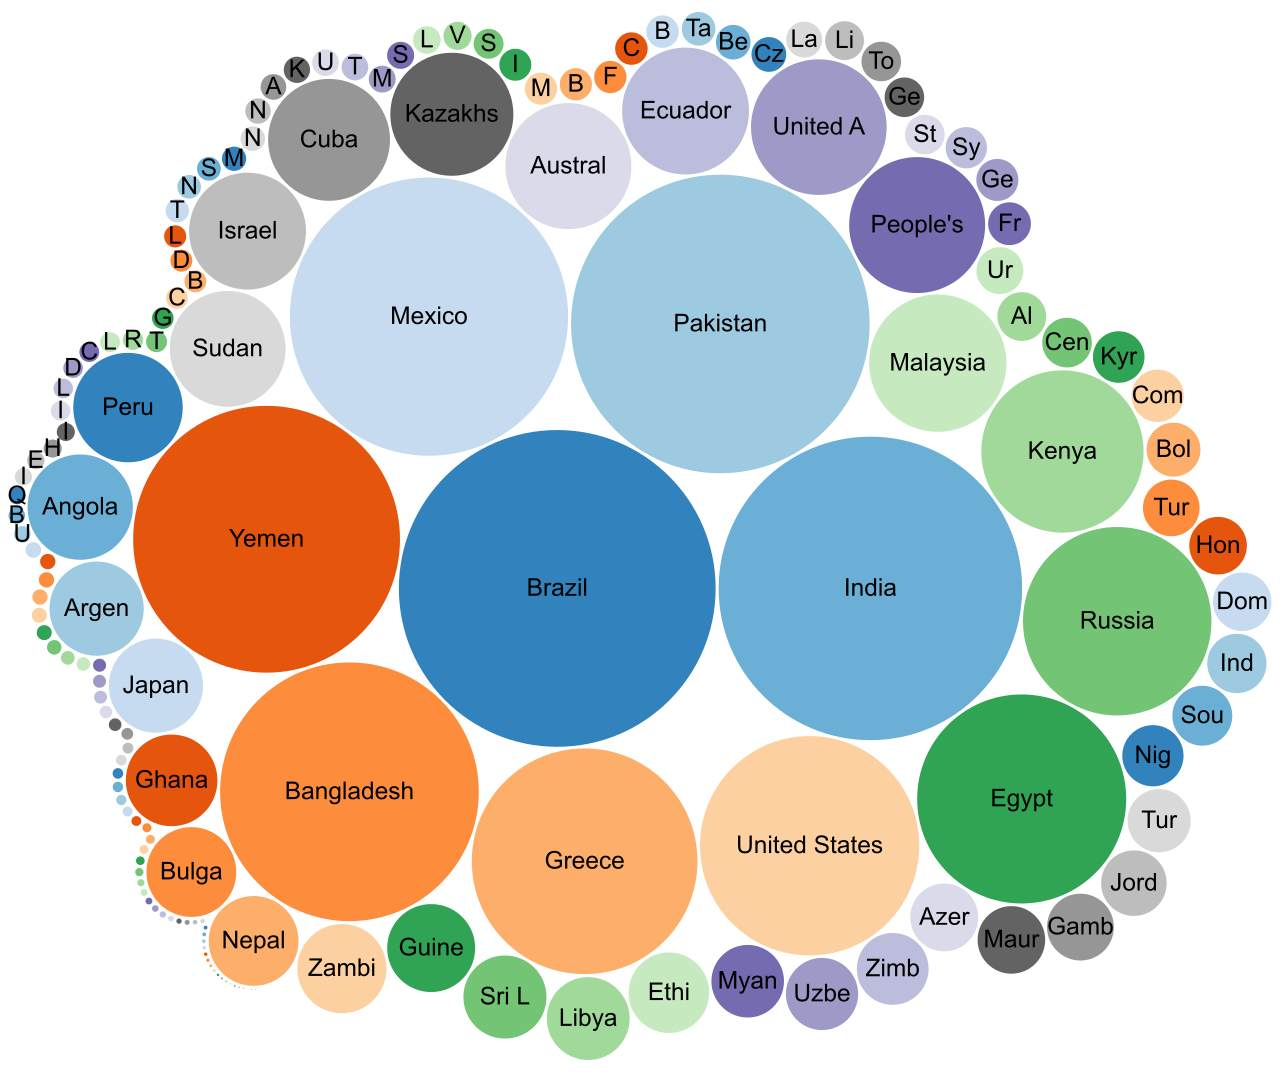
\includegraphics[width=0.94\linewidth]{./chapter/human_settlement/AnnaBubbleHumanSettlement.jpg}
    \caption[Сколько населения проживает в~населённых пунктах, 2017.]{Пузырьковая диаграмма с суммарным количеством населения,\\проживающего в~<<населённых пунктах>> на 2017 год} 
%Размер пузырька соответствует количеству населения, проживающего в~<<населённых пунктах>> одной страны. Ссылка на SPARQL-запрос: \href{https://w.wiki/4dAv}{https://w.wiki/4dAv}}
    \label{fig:human-settlement-1}
\end{marginfigure}

%\marginnote{%
%См. ответ~\ref{answer:flag_human_settlements} на с.~\pageref{answer:flag_human_settlements}.
%}
С помощью запроса~\ref{lst:human-settlement3} 
построим упорядоченный список стран по суммарному количеству населения, проживающего в~<<населённых пунктах>>.


%\begin{minipage}{\linewidth}
%\marginnote[0cm]{Получена \num{161} страна в 2017 году и \num{213} стран в 2021 году. SPARQL-запрос: \href{https://w.wiki/4d9M}{https://w.wiki/4d9M}}
\index{SPARQL!SUM}
\index{SPARQL!GROUP BY}
\lstset{numbers=left, firstnumber=1, frame=single}
\begin{lstlisting}[ 
    language=SPARQL, 
    caption={\href{https://w.wiki/4d9M}{Список стран по суммарному количеству населения, проживающего\\в~<<населённых пунктах>>}\protect\footnotemark},
    label=lst:human-settlement3,
    texcl,
    xleftmargin=18pt, 
    numbers=left]
# List of countries by population in settlements
SELECT ?country ?countryLabel (SUM(?population) as ?sumPopulation)
WHERE {
  ?hum wdt:P31 wd:Q486972;      # instance of human settlement
       wdt:P17 ?country;        # in the ?country
       wdt:P1082 ?population.   # has ?population
  SERVICE wikibase:label{bd:serviceParam wikibase:language "ru,en"}
}
GROUP BY ?country ?countryLabel 
ORDER BY DESC (?sumPopulation)
\end{lstlisting}%
\footnotetext{Получено: \num{161} страна в 2017 году и \num{213} стран в 2021 году. SPARQL-запрос: \href{https://w.wiki/4d9M}{https://w.wiki/4d9M}.}
%\end{minipage}


Для подсчёта количества населения по странам 
используем команду \lstinline|SUM()| в~строке~2 запроса~\ref{lst:human-settlement3}. 
Для группировки населённых пунктов по странам 
используем команду \lstinline|GROUP BY|\, в~строке~9 того~же запроса.

Пузырьковая диаграмма на рис.~\ref{fig:human-settlement-1} и~\ref{fig:human-settlement-2} 
показывает соотношение стран по количеству населения в~<<населённых пунктах>> 
в~2017 и~2021~годах соответственно. 
Размер пузырька соответствует количеству населения, проживающего в~<<населённых пунктах>> одной страны. 
SPARQL-запрос для~построения такой диаграммы доступен по ссылке: \href{https://w.wiki/4dAv}{https://w.wiki/4dAv}.

%\begin{fullwidth}
%\noindent\begin{minipage}[]{.46\linewidth}
%    \centering
%\begin{marginfigure}[0.0cm]
%	    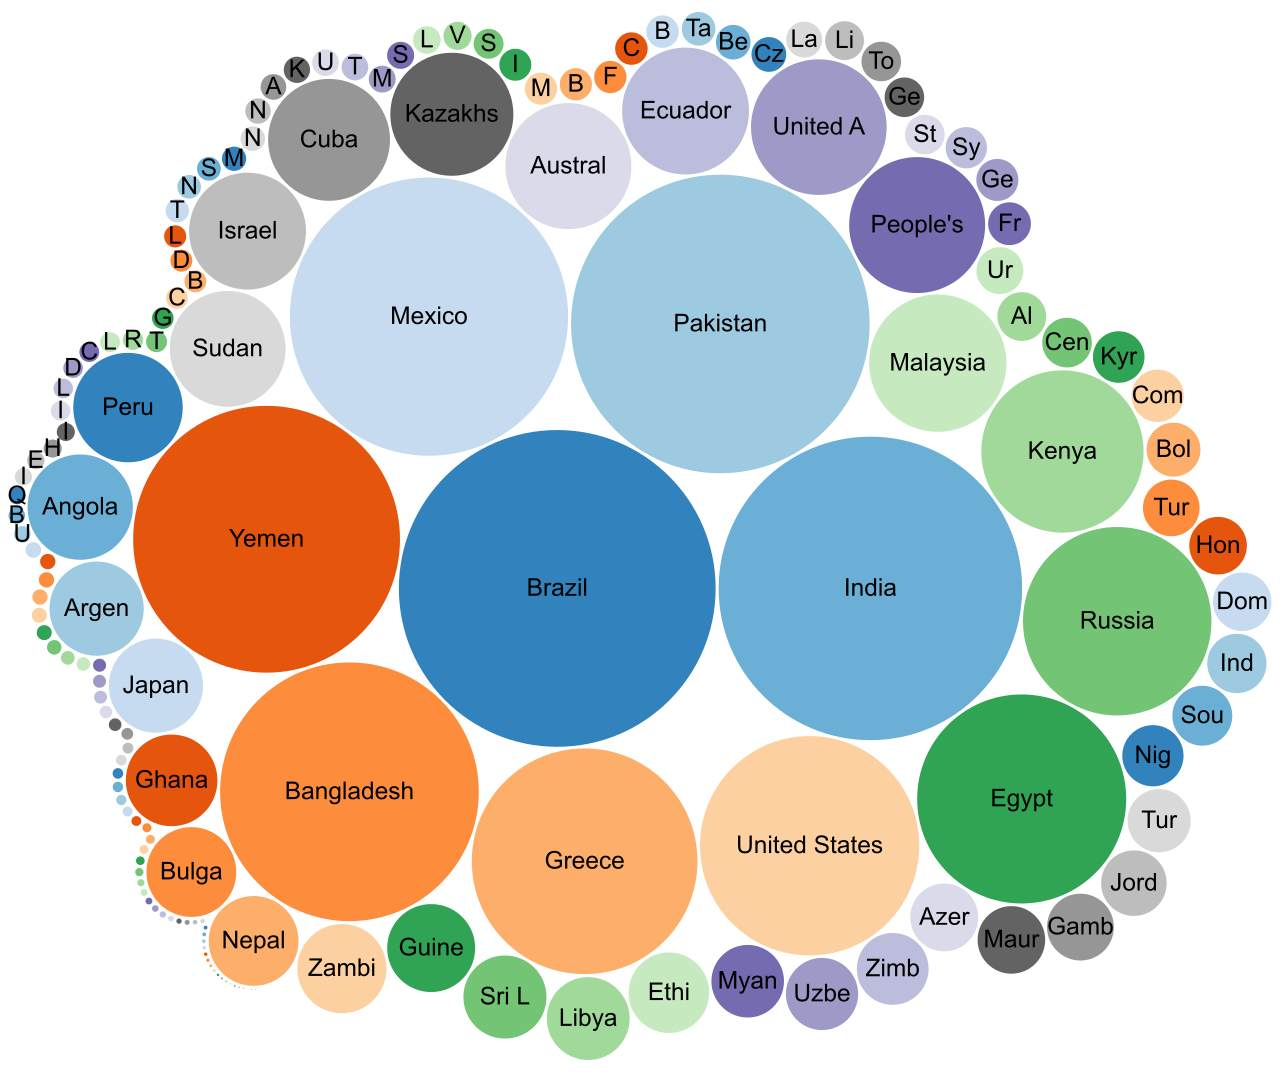
\includegraphics[width=0.94\linewidth]{./chapter/human_settlement/AnnaBubbleHumanSettlement.jpg}
%        \caption[Сколько населения проживает в~населённых пунктах, 2017.]{Пузырьковая диаграмма с суммарным количеством населения, проживающего в~<<населённых пунктах>> на 2017 год} 
        %Размер пузырька соответствует количеству населения, проживающего в~<<населённых пунктах>> одной страны. Ссылка на SPARQL-запрос: \href{https://w.wiki/4dAv}{https://w.wiki/4dAv}}
%	    \label{fig:human-settlement-1}
%\end{marginfigure}
%\end{minipage}%
%just a break for lines between two columns of listings
%\hfill
%\begin{minipage}[]{.46\linewidth}
%    \centering
\begin{marginfigure}[0.0cm]
	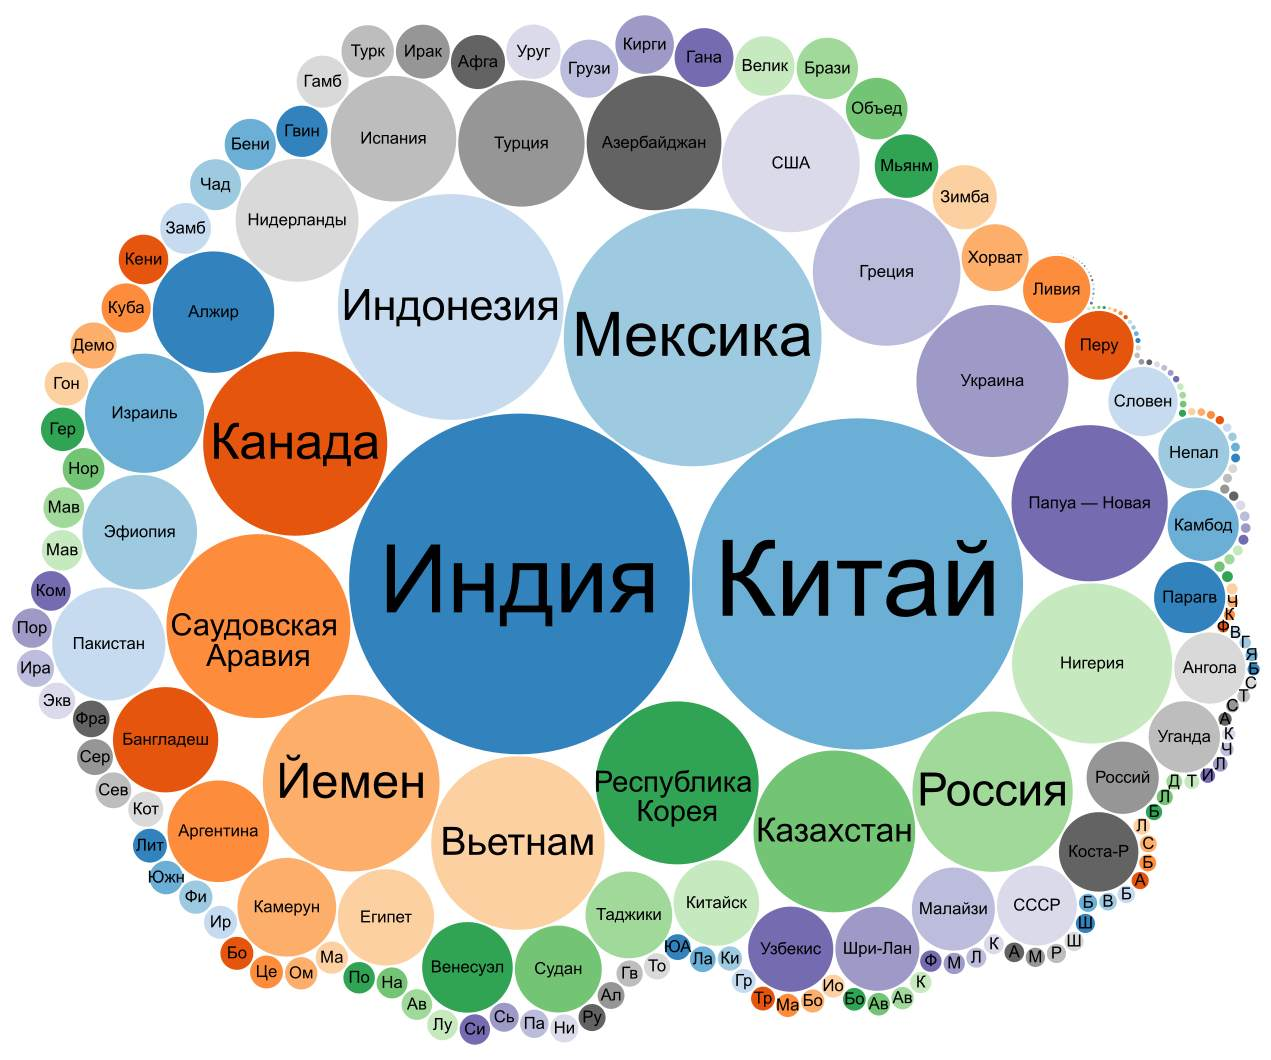
\includegraphics[width=0.75\linewidth]{./chapter/human_settlement/LeonidBubbleHumanSettlement.jpg}
    \caption[Сколько населения проживает в~населённых пунктах, 2021.]{Пузырьковая диаграмма с суммарным количеством населения,\\проживающего в~<<населённых пунктах>> на 2021 год} 
    %Размер пузырька соответствует количеству населения, проживающего в~<<населённых пунктах>> одной страны. Ссылка на SPARQL-запрос: \href{https://w.wiki/4dAv}{https://w.wiki/4dAv}}
	\label{fig:human-settlement-2}
\end{marginfigure}
%\end{minipage}
%\end{fullwidth}%



%\begin{figure}
%\centering
%	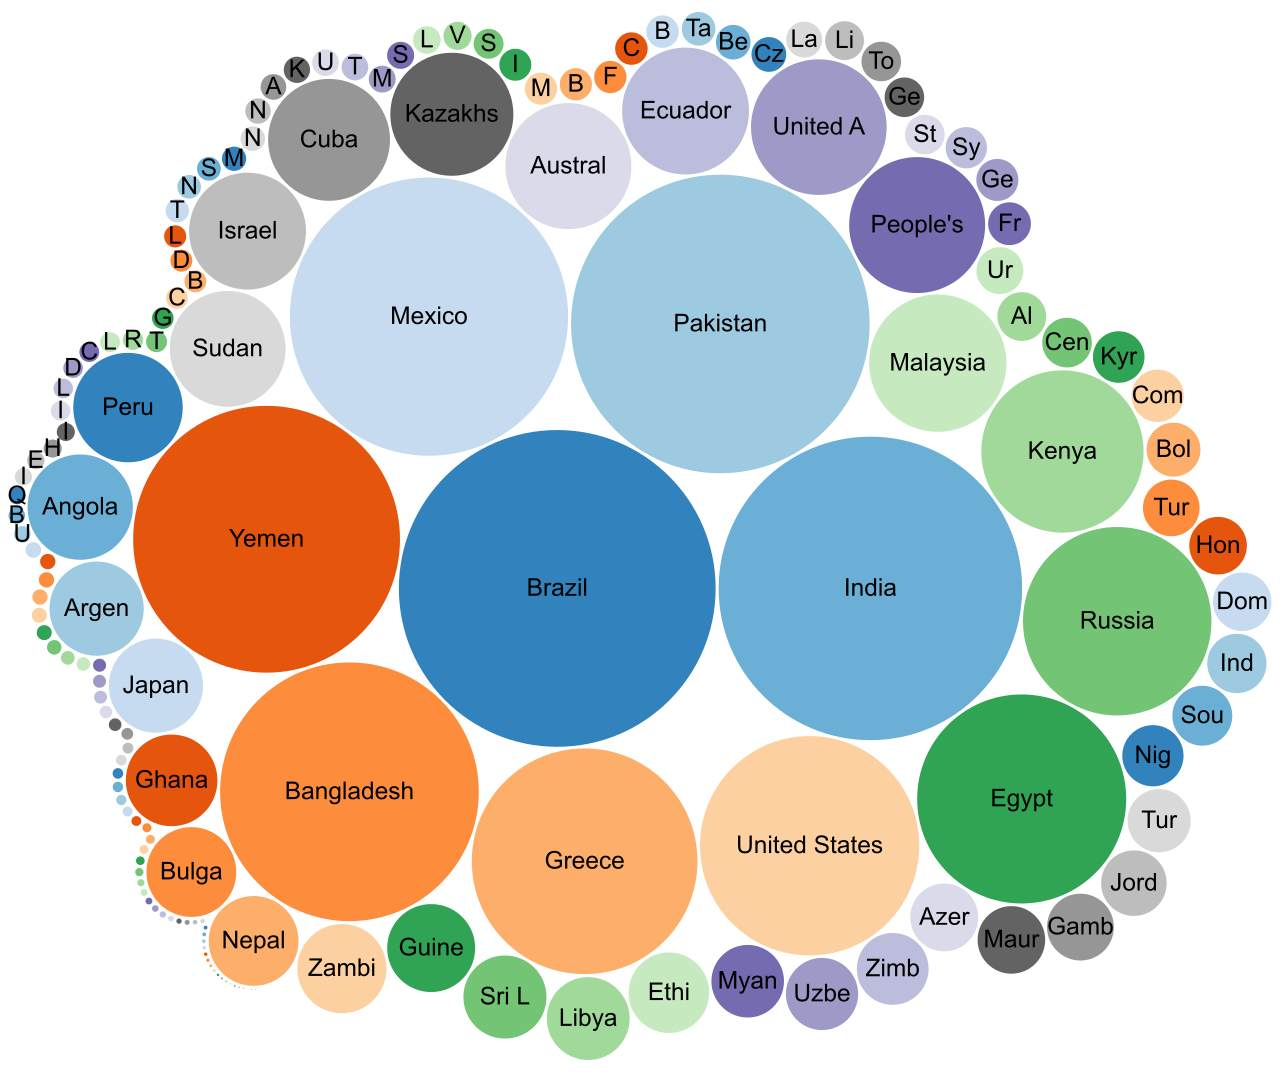
\includegraphics[width=0.9\linewidth]{./chapter/human_settlement/AnnaBubbleHumanSettlement.jpg}
%	\label{fig:human-settlement-1}
%    \caption[Пузырьковая диаграмма с суммарным количеством населения в~населённых пунктах, 2017 год.]{Пузырьковая диаграмма с суммарным количеством населения, проживающего в~<<населённых пунктах>> на 2017 год. Размер пузырька соответствует количеству населения, проживающего в~<<населённых пунктах>> одной страны. Ссылка на SPARQL-запрос: \href{https://w.wiki/4dAv}{https://w.wiki/4dAv}}
%\end{figure}

%\begin{figure}
%\centering
%	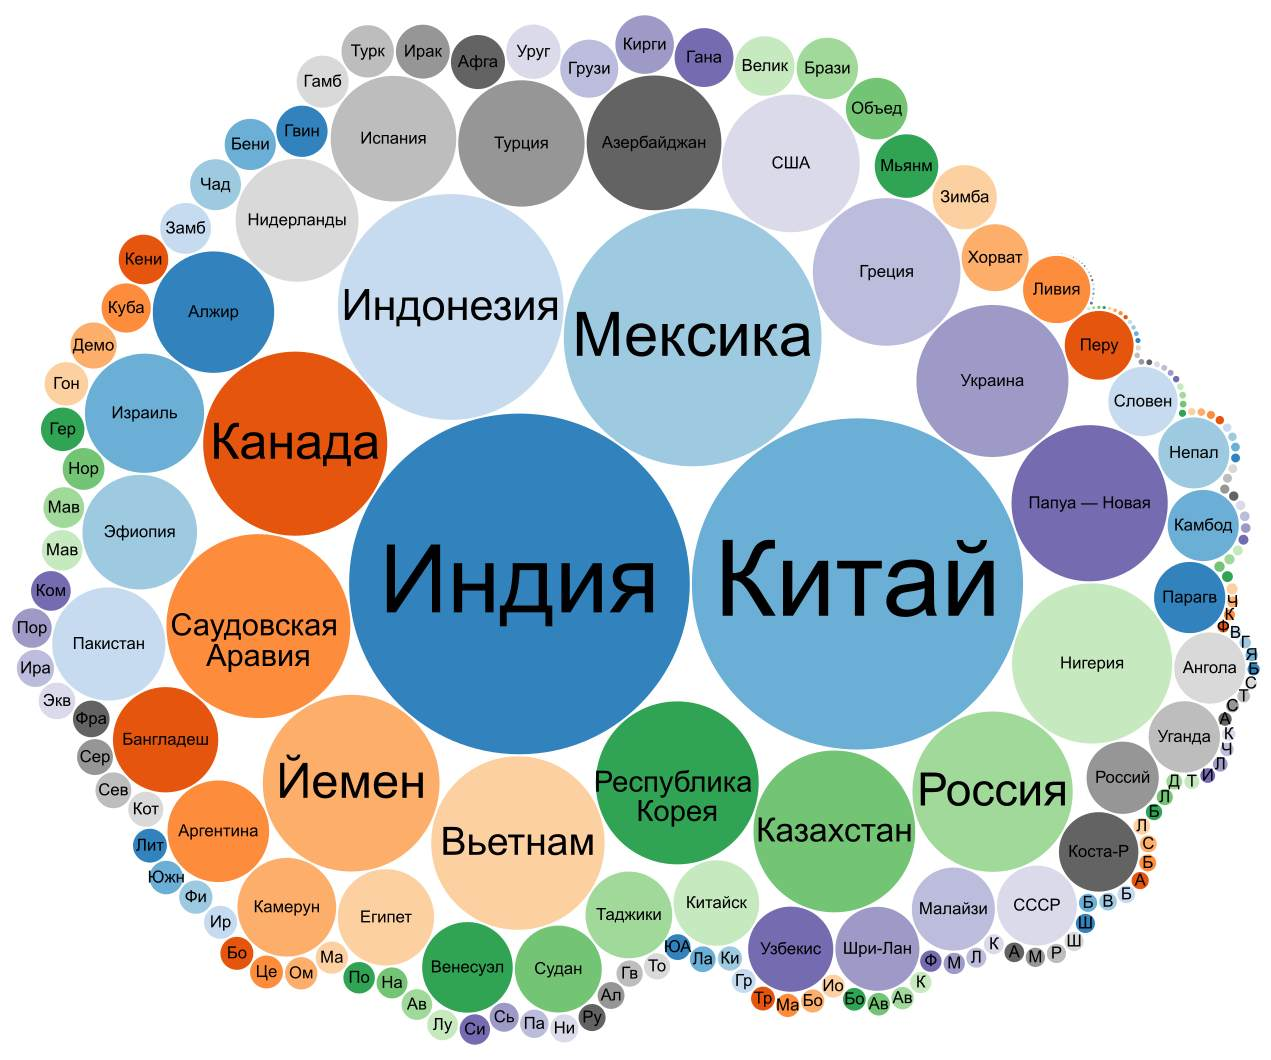
\includegraphics[width=0.9\linewidth]{./chapter/human_settlement/LeonidBubbleHumanSettlement.jpg}
%	\label{fig:human-settlement-2}
%	\caption[Пузырьковая диаграмма с суммарным количеством населения в~населённых пунктах, 2021 год.]{Пузырьковая диаграмма с суммарным количеством населения, проживающего в~<<населённых пунктах>> на 2021 год. Размер пузырька соответствует количеству населения, проживающего в~<<населённых пунктах>> одной страны. Ссылка на SPARQL-запрос: \href{https://w.wiki/4dAv}{https://w.wiki/4dAv}}
%\end{figure}

В 2017 году больше всего населения проживало в~<<населённых пунктах>> 
\wdqName{Бразилии}{155} (12~млн), 
\wdqName{Пакистана}{843} (\num{10} млн), 
\wdqName{Мексики}{96} (\num{8} млн), 
\wdqName{Йемена}{805} (\num{8} млн), 
\wdqName{Индии}{668} и 
\wdqName{Бангладеш}{902} (по \num{7} млн). 

На рис.~\ref{fig:human-settlement-2} можно увидеть список стран на 2021 год: 
\wdqName{Индия}{668} (\num{30} млн), 
\wdqName{Китай}{148} (28~млн), 
\wdqName{Мексика}{96} (\num{17} млн), 
\wdqName{Индонезия}{252} (\num{13} млн), 
\wdqName{Канада}{16} (\num{9} млн) и 
\wdqName{Саудовская Аравия}{851} (\num{9}~млн). 

Итак, результаты запроса~\ref{lst:human-settlement3} в~2017 и 2021 годах существенно разнятся. 
По этим результатам получается, что за четыре года 
в~населённых пунктах Индии стало больше на 23 млн человек. 


%%%%%
\section[Полнота Викиданных по заполненности свойств населённых пунктов]
        {Полнота Викиданных по заполненности свойств населённых пунктов}

Населённый пункт~--- это общее название мест с постоянными жителями. %\autocite{Humansettlements_Dictionary}. 
По версии редакторов Викиданных, в~понятие <<насёленный пункт>> входят города, сёла, деревни 
и другие виды поселений\sidenote[][-1\baselineskip]{%% 
    Несколько наиболее частотных классов таких поселений можно посмотреть  
      в~табл.~\ref{tab:human-settlement-classes} 
    на~с.~\pageref{tab:human-settlement-classes}.%
}. 
Точной информации о количестве населённых пунктов в~мире мы не нашли. 
Поэтому проверим полноту тех населённых пунктов, которые есть в~Викиданных 
и которые использовались для~решения задачи. 
В~задачах выше мы использовали свойства <<\wdProperty{1082}{численность населения}>> и 
<<\wdProperty{17}{государство}>> (привязка к стране). 
Исходя из этого, проверку полноты разделим на подзадачи: 
%%%%%%%%%%%%%%%% Упражнение 4 %%%%%%%%%%%%%%%%
\marginnote[-2\baselineskip]{%
    \MarginQuestion Герб населённого пункта какой страны изображён?
    \vspace{5pt}

    \includegraphics[width=2cm]{./chapter/human_settlement/Loučovice_CoA.jpg}

    См. ответ %~\ref{answer:flag_human_settlements} 
    на с.~\pageref{answer:flag_human_settlements}.%
    \label{fig:flag_question_human_settlements3}%
    \vspace{5pt}
}% eo marginnote
%%%%%
\begin{enumerate} 
  \item Проверка заполненности свойства <<численность населения>>.
  \item Проверка принадлежности к государству.
\end{enumerate}


%%%%%
\subsection{Проверка заполненности свойства <<численность населения>> }

Для такой проверки напишем \href{https://w.wiki/4FUz}{SPARQL-запрос}\sidenote{
%
    В 2017 году запрос выдал \num{372997} населённых пунктов 
    с незаполненным свойством <<численность населения>>. 
    Тот же запрос в~2021 году выдал \num{507078} таких населённых пунктов. 
    Ссылка на SPARQL-запрос: \href{https://w.wiki/4FUz}{https://w.wiki/4FUz}.% 
}, 
который выведет населённые пункты 
с незаполненным свойством <<\href{http://www.wikidata.org/entity/P1082}{численность населения}>>. 
Произведя расчёты, получили, что только у 9,3\,\% населённых пунктов мира 
было указано свойство <<численность населения>> на 2017 год. 
В~2021 году получили 11,2\,\% населённых пунктов мира с~заполненным свойство <<численность населения>>. 
Итак, одновременно с~ростом числа населённых пунктов в~Викиданных 
растёт доля пунктов с~заполненным свойством <<численность населения>>.


%%%%%
\subsection{Проверка принадлежности к государству}

А теперь посмотрим населённые пункты, 
у которых не указана принадлежность к какой-либо стране, 
с помощью \href{https://w.wiki/4FV8}{SPARQL-запроса}\footnote{%
%
    В 2017 году нашлось \num{8427} объектов, у которых не указана принадлежность к какой-либо стране. 
    В 2021 году таких объектов уже больше~--- \num{27824}. SPARQL-запрос: \href{https://w.wiki/4FV8}{https://w.wiki/4FV8}.%
}. 

Результаты запроса показывают, что число пунктов без привязки к стране растёт с~годами. 
Поэтому вычисления, связанные с~населёнными пунктами и странами, 
по определению будут неполными даже относительно тех пунктов, которые уже есть в~Викиданных. 



\section{Доля населения страны, проживающего в~<<населённых пунктах>>}

Построим список стран, 
упорядоченный по доли населения (в~процентах), проживающей в~\href{http://www.wikidata.org/entity/Q486972}{населённых пунктах}, относительно числа всех жителей страны (листинг~\ref{lst:human-settlement6}).


\index{SPARQL!SUM}
\index{SPARQL!SELECT!вложенный}
\begin{lstlisting}[ language=SPARQL, 
    caption={\href{https://w.wiki/4dE3}
                  {Соотношение количества людей, проживающих в населённых пунктах,\\
                  к количеству всех людей в стране}\protect\footnotemark},
    label=lst:human-settlement6,
    texcl,
    xleftmargin=18pt, 
    numbers=left,
    ]
# An ordered list of the ratio of the number of people living in 
# "human\_settlement" to the number of inhabitants in the country.
SELECT ?country ?countryLabel ?proportionPopulation WHERE {
 SELECT ?country ?countryLabel (SUM(?population / ?pop) 
        as ?proportionPopulation) WHERE {
  ?hum wdt:P31 wd:Q486972;    # instances of human settlement  
       wdt:P17 ?country;         # has ?country 
       wdt:P1082 ?population.    # has ?population
  ?country wdt:P1082 ?pop.    # population in the country
  SERVICE wikibase:label{bd:serviceParam wikibase:language "ru,en"}
 }
 GROUP BY ?country ?countryLabel
}
ORDER BY ?proportionPopulation
\end{lstlisting}%
%%%%%%%%%%%%%%%% Упражнение 5 %%%%%%%%%%%%%%%%
\marginnote[-15\baselineskip]{%
    \MarginQuestion Герб населённого пункта какой страны изображён?
    \vspace{5pt}

    \includegraphics[width=2cm]{./chapter/human_settlement/POL_Otynia_COA.png}
    
    См. ответ %~\ref{answer:flag_human_settlements} 
    на с.~\pageref{answer:flag_human_settlements}.%
    \label{fig:flag_question_human_settlements4}%
} 
\footnotetext{Получено: \num{158} результатов в 2017 году и \num{206} результатов в 2021 году. Ссылка на SPARQL-запрос: \href{https://w.wiki/4dE3}{https://w.wiki/4dE3}.}


Столбчатая диаграмма на рис.~\ref{fig:human-settlement-3} позволяет увидеть для~каждой страны 
отношение количества людей, 
проживающих в~\href{http://www.wikidata.org/entity/Q486972}{населённых пунктах}, 
к~числу жителей в~стране на 2017 год.
Наиболее высокий процент приходился на следующие страны: 
Кирибати (78\,\%), Ниуэ (70\,\%), Греция (53\,\%), Тувалу (48\,\%), Коморы (43\,\%), Маврикий (42\,\%). 
В 2022 году картина изменилась: Нигерия (93\,\%), Папуа~--- Новая Гвинея (71\,\%), 
Израиль (50\,\%), Греция (47\,\%), Азербайджан (47\,\%), Казахстан (37\,\%). 


Для построения аналогичной диаграммы за 2022 год (рис.~\ref{fig:human-settlement-4}) 
мы немного изменили запрос~\ref{lst:human-settlement6}, 
добавив ограничение~--- выводить страны с населением более 5~млн~человек\sidenote[][-1\baselineskip]{%
%
    Строка с ограничением:\\
    \lstinline|FILTER (?pop > 5000000).|
%
}. Таким образом, рис.~\ref{fig:human-settlement-4} построен 
с~помощью запроса \href{https://w.wiki/5Ajn}{https://w.wiki/5Ajn}. 


На 2017 год в странах большой восьмёрки доля жителей 
в \href{http://www.wikidata.org/entity/Q486972}{населённых пунктах} составила: 
\href{http://www.wikidata.org/entity/Q159}{Россия} (\num{2.98}\,\%), 
\href{http://www.wikidata.org/entity/Q30}{США} (\num{1.76}\,\%), 
\href{http://www.wikidata.org/entity/Q17}{Япония} (\num{0.80}\,\%), 
\href{http://www.wikidata.org/entity/Q16}{Канада} (\num{0.26}\,\%), 
\href{http://www.wikidata.org/entity/Q142}{Франция} (\num{0.20}\,\%), 
\href{http://www.wikidata.org/entity/Q183}{Германия} (\num{0.24}\,\%), 
\href{http://www.wikidata.org/entity/Q145}{Великобритания} (\num{0.18}\,\%), 
\href{http://www.wikidata.org/entity/Q38}{Италия} (\num{0.07}\,\%). 
В 2022 году значения доли населения снизились (рис.~\ref{fig:human-settlement-4}): 
\href{http://www.wikidata.org/entity/Q159}{Россия} (0.045\,\%), 
\href{http://www.wikidata.org/entity/Q30}{США} (\num{0.014}\,\%), 
\href{http://www.wikidata.org/entity/Q17}{Япония} (\num{0.008}\,\%), 
\href{http://www.wikidata.org/entity/Q16}{Канада} (\num{0.23}\,\%), 
\href{http://www.wikidata.org/entity/Q142}{Франция} (\num{0.005}\,\%), 
\href{http://www.wikidata.org/entity/Q183}{Германия} (\num{0.005}\,\%), 
\href{http://www.wikidata.org/entity/Q145}{Великобритания} (\num{0.014}\,\%), 
\href{http://www.wikidata.org/entity/Q38}{Италия} (\num{0.0005}\,\%). 
Отметим, что это страны промышленно развитые.

\begin{figure*}
    \includegraphics[width=1\linewidth]{./chapter/human_settlement/AnnaShareHumanSettlement.png}
	\label{fig:human-settlement-3}
	\caption[Доля населения страны, проживающего в населённых пунктах, 2017 год.]{Доля населения страны, проживающего в~<<населённых пунктах>>, 2017 год. Ссылка на SPARQL-запрос: \href{https://w.wiki/4dE3}{https://w.wiki/4dE3}}%
\end{figure*} 


\begin{figure*}
% see https://commons.wikimedia.org/wiki/File:Proportion_of_the_country%27s_population_living_in_human_settlements_for_2022.png    
    \includegraphics[width=1\linewidth]{./chapter/human_settlement/ShareHumanSettlement_2022.png}
	\label{fig:human-settlement-4}
	\caption[Доля населения страны, проживающего в населённых пунктах, 2022 год.]
            {Доля населения страны, проживающего в~<<населённых пунктах>>, 2022 год. 
            Выбраны страны с~населением более 5~млн~чел. 
            SPARQL-запрос: \href{https://w.wiki/92jq}{https://w.wiki/92jq}}%
\end{figure*}%

Отметим некоторую закономерность, которую показывают эти диаграммы, а именно: 
чем более развита страна, тем меньшая доля людей проживает в~объектах типа 
<<\wdqName{населённый пункт}{486972}>>. 
По-видимому, рис.~\ref{fig:human-settlement-3} и~\ref{fig:human-settlement-4} 
подсказывают нам, что в таких странах население в~основном проживает 
в~поселениях другого типа. Осталось найти, что это за~поселения. 





%%%%%
\section[Cписок классов, сопутствующих <<населённому пункту>> в~свойстве <<экземпляр>>]{Cписок классов, сопутствующих <<населённому пункту>>\\в~свойстве <<экземпляр>>}
\label{human-settlement:tag1}

%%%%%%%%%%%%%%%% Упражнение 6 %%%%%%%%%%%%%%%%
\marginnote{%
    \MarginQuestion Герб населённого пункта какой страны изображён?
    \vspace{5pt}

    \includegraphics[width=2cm]{./chapter/human_settlement/Coat_of_Arms_of_Azov.png}

    См. ответ %~\ref{answer:flag_human_settlements} 
    на с.~\pageref{answer:flag_human_settlements}.%
    \label{fig:flag_question_human_settlements5}%
} 
Будем называть <<классом>> такие объекты Викиданных, 
которые связаны с~каким-либо объектом Викиданных посредством свойства \wdProperty{31}{экземпляр}. 
Цель этого раздела~--- найти объекты $X$, 
для~которых объект <<\wdqName{населённый пункт}{486972}>> является \emph{классом}, 
и получить другие классы объекта $X$, кроме <<населённого пункта>>. 
Эти <<другие>> классы будем называть сопутствующими <<населённому пункту>>. 
С помощью запроса~\ref{lst:human-settlement7} 
найдём объекты, сопутствующие <<населённому пункту>>. 



%\marginnote[1cm]{Получено 610 результатов в 2017 году и \num{1245} результатов в 2021 году. SPARQL-запрос: \href{https://w.wiki/4dEW}{https://w.wiki/4dEW}}
\begin{lstlisting}[ language=SPARQL, 
    caption={\href{https://w.wiki/4dEW}{Cписок объектов, сопутствующих <<населённому пункту>>}\protect\footnotemark},
    label=lst:human-settlement7,
    texcl,
    xleftmargin=18pt, 
    numbers=left,
    ]
# List of classes accompanying the human\_settlement (instance of)
SELECT ?inst (COUNT(?hum) as ?sumHum) 
WHERE{          
  ?hum wdt:P31 wd:Q486972; # instance of human settlement
       wdt:P31 ?inst.      # other objects in instance
  SERVICE wikibase:label{bd:serviceParam wikibase:language "ru,en"}
}  
GROUP BY ?inst
\end{lstlisting}%
\footnotetext{Получено: 610 результатов в 2017 году и \num{1245} результатов в 2021 году. SPARQL-запрос: \href{https://w.wiki/4dEW}{https://w.wiki/4dEW}.}

Для ускорения выполнения запроса~\ref{lst:human-settlement7} выполним два шага.
 
Во-первых, выключим из рассмотрения поселения, 
имеющие в~списке экземпляров только <<населённый пункт>>, 
поскольку тогда других сопутствующих классов нет. 
Для этого добавим в~запрос~\ref{lst:human-settlement8} строку~\num{9} с~фильтром, 
требующим, чтобы у объекта \lstinline|?hum|, 
кроме \wdProperty{31}{экземпляра} <<\wdqName{населённый пункт}{486972}>>, был ещё какой-либо класс.

Во-вторых, в~строке \num{8} запроса~\ref{lst:human-settlement8} 
уберём такие объекты переменной \lstinline|?inst|, 
которые имеют свойство <<\wdqName{государство}{17}>>. 
Это позволит отсечь сотни типов населённых пунктов, специфичных для~отдельных стран, 
например <<административно-территориальная единица России>>.

Эти преобразования позволили выполнить запрос~\ref{lst:human-settlement8} 
по всем странам мира за~13~мс, что является вполне приемлемым временем.


\newpage
\lstset{numbers=left, firstnumber=1, frame=single}
\begin{lstlisting}[ language=SPARQL, 
    caption={\href{https://w.wiki/4ePf}{Cписок классов, сопутствующих <<населённому пункту>> в~свойстве <<экземпляр>> без~специализированных классов разных стран}\protect\footnotemark},
    label=lst:human-settlement8,
    texcl,
    xleftmargin=18pt, 
    numbers=left,
    ]
# List of objects with the class of human settlement, without 
# country and single human settlement
SELECT ?inst ?instLabel (COUNT(?hum) as ?sumHum) 
WHERE{ 
  ?hum wdt:P31 wd:Q486972;  # instance of human settlement
       wdt:P31 ?inst.       # other objects in instance
  
  MINUS {?inst wdt:P17 []}. # without country
  FILTER(?inst != wd:Q486972 ). # without human settlement
  SERVICE wikibase:label{bd:serviceParam wikibase:language "ru,en"}
}  
GROUP BY ?inst ?instLabel
ORDER BY DESC (?sumHum)
\end{lstlisting}%
\footnotetext{Получено: 355 записей в 2017 году и 707 записей в 2021 году. Ссылка на~SPARQL-запрос: \href{https://w.wiki/4ePf}{https://w.wiki/4ePf}.}

В табл.~\ref{tab:human-settlement-classes} представлены классы, 
сопутствующие <<населённому пункту>> в~свойстве <<экземпляр>>, 
и~сравнение количества этих классов за 2017 и 2021 годы. 
Получены данные по всему миру, представлены первые строки ответа на запрос~\ref{lst:human-settlement9}.

\begin{margintable}[0.0cm]
%\begin{table}[h]
%\footnotesize
%\centering

\caption[Сопутствующие населённому пункту классы, 2017 и 2021 годы.]
        {Сопутствующие <<населённому пункту>> классы, 2017 и 2021 годы%, их разница ($\Delta$)
        \vspace{1pt}}
\begin{tabular}{|l|l|l|l|l|}
\hline
\textnumero & Класс населённого пункта   & 2017 & 2021 & $\Delta$ \\ \hline
1 & \wdqName{Cело}{532}                  & \num{2844}       & \num{4853} & +\num{2009}	\\
2 & \wdqName{Муниципалитеты}{15284}      & \num{1181}       & \num{3376} & +\num{2195}	\\
3 & \wdqName{Деревни}{5084}              & \num{662}        & \num{1761} & +\num{1099}	\\ 
4 & \wdqName{Археологические памятники}{839954}	& \num{425} & \num{887}	& +\num{462}	\\ 
5 & \wdqName{Местные поселения}{3257686} & \num{425}        & \num{158}	& -\num{257}	\\ 
6 & \wdqName{Разрушенные города}{14616455} & \num{423}      & \num{388}	& -\num{40}	\\
7 & \wdqName{Города}{515}                 & \num{322}       & \num{545}	& +\num{223}	\\
8 & \wdqName{Малые города}{3957}		  & \num{277}       & \num{446}	& +\num{169}	\\ 
9 & \wdqName{Заброшенные деревни}{350895} & \num{254}       & \num{474}	& +\num{220}	\\ 
10 & \wdqName{Внутренние районы}{2983893} & \num{207}       & \num{503}	& +\num{296}	\\ \hline
\end{tabular}
\label{tab:human-settlement-classes}
%\end{table}   
\end{margintable}


Запрос~\ref{lst:human-settlement8} показал, что на 2021 год на первых местах 
среди сопутствующих <<населённому пункту>> классов 
были %доисторические поселения трёх типов: 
поселения 
\wdqName{<<латенского периода>>}{106505016}, 
\wdqName{<<бронзового века>>}{106491277} 
и поселения \wdqName{<<доисторического времени, где есть письмен\-ность>>}{106505070}. 

Попробуем сформулировать запрос так, чтобы отсечь всё множество доисторических поселений.  
Что есть общего у этих трёх объектов на Викиданных? 
Они являются экземплярами объектов, которые, в~свою очередь, 
являются экземплярами объектов \wdqName{<<археологической культуры>>}{465299}, 
\wdqName{<<исторического периода>>}{11514315}, 
\wdqName{<<археологического века>>}{15401699}, 
\wdqName{<<всемирной истории>>}{200325} 
и \wdqName{<<геологического периода>>}{392928}. 
Применим такой фильтр в~запросе~\ref{lst:human-settlement9} в~строках 11--12, 
чтобы отсечь именно эти типы объектов.

В итоге 707 классов запроса~\ref{lst:human-settlement8} 
мы сократили в~запросе~\ref{lst:human-settlement9} 
до 89 различных классов, сопутствующих <<населённому пункту>> в~свойстве <<экземпляр>>. 
В табл.~\ref{tab:human-settlement-classes} были представлены 
первые 10 наиболее частотных классов из 89. 



\newpage
%\begin{fullwidth}
\index{SPARQL!COUNT}
\index{SPARQL!FILTER}
\index{SPARQL!MINUS}
\lstset{numbers=left, firstnumber=1, frame=single}
\begin{lstlisting}[ language=SPARQL, 
    caption={\href{https://w.wiki/5AdW}{Cписок классов, сопутствующих <<населённому пункту>> в~свойстве <<экземпляр>>,\\без~исторических объектов}\protect\footnotemark},
    label=lst:human-settlement9,
    texcl,
    xleftmargin=18pt, 
    numbers=left,
    ]
# List of classes accompanying the human\_settlement in the property 'instance of' 
# without historical objects 
SELECT ?inst ?instLabel (COUNT(?hum) as ?sumHum)
WHERE{
  ?hum wdt:P31 wd:Q486972;    # instance of human settlement
       wdt:P31 ?inst.         # other objects in instance of human settlement
  ?inst wdt:P31 [wdt:P31 ?typ]. # instance of instance
  MINUS {?inst wdt:P17 []}.   # without country

  # without human settlement and prehistoric settlements
  FILTER(?inst != wd:Q486972 && ?typ != wd:Q465299 && ?typ != wd:Q11514315 
         && ?typ != wd:Q15401699 && ?typ != wd:Q200325 && ?typ != wd:Q392928). 

  SERVICE wikibase:label{bd:serviceParam wikibase:language "ru,en"}
}
GROUP BY ?inst ?instLabel
ORDER BY DESC (?sumHum)
\end{lstlisting}%
\footnotetext{Получено: 89 результатов. Ссылка на SPARQL-запрос: \href{https://w.wiki/5AdW}{https://w.wiki/5AdW}.}
%\end{fullwidth}




%%%%%
\section{Отечественные учёные на селе и в городе}

Подсчитаем и сравним число отечественных учёных, родившихся в~сельских и городских типах населённых пунктов. 
Решим эту задачу в~пять шагов:
\begin{enumerate}
  \item Выявим список сельских и список городских типов поселений именно в~России.
  \item Определим основные научные направления, представленные в~Викиданных.
  \item Выявим способ определения отечественных учёных.
  \item Сделаем такую диаграмму, на которой разным цветом будут указаны разные научные направления (математики, физики, химики и так далее) для~учёных, родившихся в~\emph{сельских поселениях}.
  \item Сделаем аналогичную диаграмму по \emph{городским поселениям} и сравним результаты.
\end{enumerate}




\newpage
%%%%%
\section{Список сельских и список городских типов поселений в~России}%
\label{sec:list-village-city-types-in-Russia}

С помощью запроса~\ref{lst:human-settlement-noname-count} 
выведем список типов поселений и их количество для~объектов, 
имеющих свойство \wdProperty{1082}{<<численность населения>>} 
и принадлежащих \wdqName{России}{159}. 

\marginnote[64pt]{%
%
    \MarginQuestion 
    Используя команду \texttt{FILTER~NOT~EXISTS},\, 
    измените запрос~\ref{lst:human-settlement-noname-count} так, чтобы получить число классов 
    с~пустым полем <<численность населения>>. 

{\noindent}См. пример использования этой команды в запросе~\ref{lst:anime_no_pub_date} 
на с.~\pageref{lst:anime_no_pub_date}.%
%
}% eo marginnote
\index{SPARQL!COUNT}
\index{SPARQL!SELECT!вложенный}
\index{SPARQL![]!безымянная переменная}
\begin{lstlisting}[ language=SPARQL, 
    caption={\href{https://w.wiki/4zPi}{Список классов поселений и их количество для объектов, имеющих свойство <<численность населения>> в России}\protect\footnotemark},
    label=lst:human-settlement-noname-count,
    texcl,
    xleftmargin=18pt, 
    numbers=left,
    ]
# List of instances of settlement with population in Russia
SELECT ?class ?classLabel (COUNT(?class) AS ?count) WHERE {
  SELECT ?class ?classLabel WHERE {
    [] wdt:P31 ?class; # noname instance of class
         wdt:P17 wd:Q159;  # in Russia
         wdt:P1082 [].     # has population
    FILTER(?class != wd:Q486972).# skip settlement itself
    SERVICE wikibase:label{bd:serviceParam wikibase:language "ru"}
  }
}
GROUP BY ?class ?classLabel
ORDER BY DESC (?count)
\end{lstlisting}%
\footnotetext{Получено: 229 разных классов поселений в 2022 году. Ссылка на SPARQL-запрос: \href{https://w.wiki/4zPi}{https://w.wiki/4zPi}.}

Из~229 классов поселений, полученных с~помощью запроса~\ref{lst:human-settlement-noname-count}, 
были выбраны те, которых много, 
и такие, которые можно уверенно отнести к~сельским или городским населённым пунктам. 
11 таких первых поселений 
представлены в~табл.~\ref{tab:human-settlement-Russia}. 
    Число в~столбце <<\textnumero>> указывает номер строки с~классом поселения 
    в~списке из 229 ответов на запрос~\ref{lst:human-settlement-noname-count}, 
    упорядоченных по их количству.



\begin{margintable}
%\centering
    \caption[Сельские и городские населённые пункты, 2022 год.]
    {Сельские и городские населённые пункты России, 2022 год%
     %Классы и количество их упоминаний среди объектов, 
     %имеющих свойство <<численность населения>> в~России
     \vspace{3pt}}
\begin{tabular}{|r|l|c|c|}
\hline
\textnumero & Название класса & \specialcell{Количество} & Население \\ \hline
1 &\specialcell{Сельское поселение\\в России (\wdq{634099})}& \num{18103} & \num{34} млн \\
2 & \wdqName{Деревня}{5084}   & \num{15517}   & \num{1,8} млн\\
3 & \wdqName{Село}{532}	      & \num{10204}   & \num{10,9} млн\\ 
4 & \wdqName{Посёлок}{2514025} & \num{4536}   & \num{3,4} млн\\ 
7 & \wdqName{Хутор}{2023000}  & \num{1782}    & \num{0,52} млн\\ 
\rowcolor{LightCyan} 
8 &\specialcell{Городское поселение\\в России (\wdq{2661988})}& \num{1502} & \num{20.0} млн \\
\rowcolor{LightCyan} 
9 & \wdqName{Город}{7930989}  & \num{1170}    & \num{103.6} млн\\ 
11 & \wdqName{Рабочий посёлок}{20019082} & \num{583} & \num{3,7} млн\\ 
13 & \wdqName{Станица}{748331} & \num{255}    & \num{1,5} млн \\
\rowcolor{LightCyan} 
20 &\specialcell{Город с населением более\\\num{100000} человек (\wdq{1549591})}& \num{107} & \num{58} млн \\
\rowcolor{LightCyan} 
55 & \wdqName{Город-миллионер}{1637706} & \num{14}    & \num{32.1} млн \\ \hline
\end{tabular}
\label{tab:human-settlement-Russia}
\end{margintable}

Обратите внимание на безымянные переменные (\lstinline|[]|) 
в строках 4~и~6 запроса~\ref{lst:human-settlement-noname-count}. 
Эта безымянность связана с~тем, что 
важен факт указания численности населения, но~не~количество людей в~них (строка~6),  
нам не нужны названия сёл и деревень (строка~4).  

Наличие строки~6 в~запросе~\ref{lst:human-settlement-noname-count} 
(\lstinline|wdt:P1082 []|) 
существенно уменьшает числа в~табл.~\ref{tab:human-settlement-Russia} 
в~столбце <<Количество>>. 
Это связано с~тем, что у многих населённых пунктов 
не~заполнено поле <<численность населения>>. 

Объект Викиданных <<\wdqName{населённый пункт}{486972}>> 
может быть указан в~качестве класса (свойство <<\wdProperty{31}{экземпляр}>>) 
как у сельских, так и у городских поселений. 
Поэтому он нам не поможет в~различении этих типов поселений 
и мы его пропускаем с~помощью строки~7 запроса~\ref{lst:human-settlement-noname-count}.



\newpage
Выберем из табл.~\ref{tab:human-settlement-Russia} строки без подсветки, 
то есть классы под номерами 1, 2, 3, 4, 7, 11 и 13. 
В~дальнейшем комбинацию этих классов будем называть \emph{сельскими поселениями}. 
%Подсчитаем, сколько всего людей живёт в таких поселениях в России. 
Подсчёты показывают, что в~таких поселениях в~России живёт 
\num{55,6} млн человек\footnote{%
Ссылка на SPARQL-запрос: \url{https://w.wiki/4$D6}.%
}. 

Суммарное число жителей по каждому из классов \emph{сельских поселений} 
вычислим с~помощью запроса~\ref{lst:human-settlement-village-count}. 
Полученные числа представлены в~табл.~\ref{tab:human-settlement-Russia} в~столбце <<Население>>. 
Если запрос~\ref{lst:human-settlement-village-count} выполняется слишком долго, 
вы можете закомментировать или удалить часть классов в~строках 3--4 
и тем самым упростить и ускорить обработку запроса. 

\index{SPARQL!VALUES}
\index{SPARQL![]!безымянная переменная}
\begin{lstlisting}[ language=SPARQL, 
    caption={\href{https://w.wiki/4$8w}{Список классов сельских поселений в~России и суммарное число жителей\\
                                        по~каждому классу}\protect\footnotemark},
    label=lst:human-settlement-village-count,
    texcl,
    xleftmargin=18pt, 
    numbers=left,
    ]
# Number of population living in villages
SELECT ?village ?villageLabel (SUM(?population) AS ?count) WHERE {  
  VALUES ?village {wd:Q634099 wd:Q5084 wd:Q532 wd:Q2514025 
                   wd:Q2023000 wd:Q20019082 wd:Q748331}
  [] wdt:P17 wd:Q159;  # settlement in the Russia
     wdt:P1082 ?population; # has ?population
     wdt:P31 ?village. # instance of ?village (see the list)
 SERVICE wikibase:label{bd:serviceParam wikibase:language "ru"}
}
GROUP BY ?village ?villageLabel
\end{lstlisting}%
\footnotetext{Число жителей в сельских поселениях России в 2022 году представлено 
в~табл.~\ref{tab:human-settlement-Russia} в~столбце <<Население>>. Ссылка на SPARQL-запрос: \url{https://w.wiki/4$8w}.}



Набор классов под номерами 8, 9, 20 и 55 в~табл.~\ref{tab:human-settlement-Russia} 
назовём \emph{городскими поселениями}. 
Подсчитаем общее число жителей в~городских поселениях России 
с~помощью запроса~\ref{lst:human-settlement-count-total-city}. 


\begin{lstlisting}[ language=SPARQL, 
    caption={\href{https://w.wiki/4$D9}{Суммарное число жителей в~городских поселениях России}\protect\footnotemark},
    label=lst:human-settlement-count-total-city,
    texcl,
    xleftmargin=18pt, 
    numbers=left,
    ]
# Number of population living in cities
SELECT (SUM(?population) AS ?count) WHERE {  
  SELECT DISTINCT ?city ?population WHERE {  
    VALUES ?city_list {wd:Q7930989 wd:Q2661988 wd:Q1549591 wd:Q1637706}
    ?city wdt:P17 wd:Q159;       # settlement in Russia
          wdt:P1082 ?population; # has ?population
          wdt:P31 ?city_list.    # instance of ?city
  }
}
\end{lstlisting}%
\footnotetext{Число жителей в городских поселениях России в~2022 году составило \num{116,1}~млн человек. 
Ссылка на SPARQL-запрос: \href{https://w.wiki/4$D9}{https://w.wiki/4\$D9}.}

Суммарное число жителей по каждому из классов \emph{городских поселений} 
вычисляется аналогично запросу~\ref{lst:human-settlement-village-count}. 
Полученные числа представлены в~табл.~\ref{tab:human-settlement-Russia} в~столбце <<Население>>. 

Таким образом, получили, что \num{55.6} млн человек живёт в~сельских поселениях и \num{116.1}~млн человек~--- в~городских. 
Общее число составило \num{171.7} млн человек, 
при этом, по оценке Росстата, в~России было 145 млн человек на 2022 год. 
Получили на 27 млн человек больше, и это с~учётом~того, что Викиданные достаточно неполные. 

На наш взгляд, проблема подсчётов заключается в~том, 
что большие города включают в~себя множество небольших городков и жители этих городков считаются дважды. 
Команда \lstinline|DISTINCT|%
%
%
\index{SPARQL!DISTINCT}
\sidenote{Команда \texttt{DISTINCT} в~строке~3 запроса~\ref{lst:human-settlement-count-total-city} 
нужна для~учёта случаев, когда одному населённому пункту \texttt{?city} 
соответствует несколько значений списка \texttt{?city\_list} в~строке~7. 
То есть населённый пункт может одновременно быть \wdProperty{31}{экземпляром} 
и~\wdqName{города}{7930989}, и~\wdqName{города-миллионера}{1637706}. 

Команда \texttt{DISTINCT} во~внутреннем цикле \texttt{SELECT} (строки~3--8) 
позволяет получить эти города (\texttt{?city}) без~дублирования. 
Если убрать слово \texttt{DISTINCT}, % из~запроса, 
то~численность населения вырастет со \num{116.1} млн до \num{187.2} млн человек. 

Отметим, что если сложить численность разных типов городов в~табл.~\ref{tab:human-settlement-Russia}, 
то~получим $20 + 103.6 + 58 + 32.1 = 213.7$. 
Очевидно, что списки разных типов городских поселений пересекаются, поэтому получилось такое большое число.%
} 
%
%
в запросе~\ref{lst:human-settlement-count-total-city} 
эту проблему не решает, поскольку большой город и входящий в~него маленький город~--- это разные объекты. 
Один из вариантов решения заключается в~том, 
чтобы дополнительно проверять населённые пункты~---  
не входят ли они в~более крупные населённые пункты, 
a~если~входят, то~не~считать их население повторно. 



%%%%%
\section{Профессии, представленные в Викиданных}

Получим список профессий и количество работников, 
имеющих российское гражданство. 
Этим запросом~\ref{lst:human-settlement13} 
мы ищем такие объекты Викиданных, 
у которых есть свойство <<\wdProperty{27}{гражданство}>> 
и~значением этого свойства является объект <<\wdqName{Россия}{159}>>. 
Очевидно, что объект, имеющий свойство <<гражданство>>, будет человеком, 
а~в~терминологии вики-проектов~--- персоной. 


\index{SPARQL!COUNT}
\lstset{numbers=left, firstnumber=1, frame=single}
\begin{lstlisting}[ language=SPARQL, 
    caption={\href{https://w.wiki/4daC}{Список профессий или должностей граждан России}\protect\footnotemark},
    label=lst:human-settlement13,
    texcl,
    xleftmargin=18pt, 
    numbers=left,
    ]
# List of occupation or job citizens of Russia 
SELECT DISTINCT ?job ?jobLabel (COUNT(?hum) AS ?count) WHERE {
  ?hum wdt:P27 wd:Q159; # citizen of Russia 
       wdt:P106 ?job. # has occupation or job
  SERVICE wikibase:label{bd:serviceParam wikibase:language "ru,en"}
}
GROUP BY ?job ?jobLabel
ORDER BY ?count
\end{lstlisting}%
\footnotetext{Получено: 2023 профессии на 2022 год. Ссылка на SPARQL-запрос: \href{https://w.wiki/4daC}{https://w.wiki/4daC}.}







\newpage
В табл.~\ref{tab:human-settlement3} представлены такие профессии  
из~результата запроса~\ref{lst:human-settlement13}, 
которые могут соответствовать каким-либо научными направлениям.


\begin{margintable}
%\centering
\caption{Научные направления и число отечественных специалистов, 2022 год}
\begin{tabular}{|r|l|c|}
\hline
\textnumero & Профессия (объект) & Число людей \\ \hline
1 & \wdqName{Физик}{169470}     & \num{991} \\
2 & \wdqName{Историк}{201788}   & \num{913} \\
3 & \wdqName{Экономист}{188094}	& \num{880} \\ 
4 & \wdqName{Математик}{170790}	& \num{857} \\ 
5 & \wdqName{Инженер}{81096}	& \num{558} \\ 
7 & \wdqName{Химик}{593644}		& \num{439} \\ 
8 & \wdqName{Врач}{39631}		& \num{342} \\ 
9 & \wdqName{Юрист}{185351}		& \num{330} \\ 
10 & \wdqName{Биолог}{864503}	& \num{222} \\ \hline
\end{tabular}
\label{tab:human-settlement3}
\end{margintable}




%%%%%
\section{Найти учёных среди людей}

Есть два способа получения списка учёных. 
Первый: у большинства учёных в~Викиданных заполнено свойство <<\wdProperty{512}{научная степень}>>. 
Запросим в~Викиданных россиян, имеющих такое свойство (запрос~\ref{lst:human-settlement14}), 
и получим список отечественных учёных. 


Отметим, что если учёный жил и в~СССР, и в~современной России, 
то у персоны в~поле <<\wdProperty{27}{гражданство}>> будут указаны обе страны.  
Благодаря команде \lstinline|DISTINCT| (строка~2 запроса~\ref{lst:human-settlement14}) 
такой учёный посчитается ровно один раз. 
Поэтому удаление команды \lstinline|DISTINCT| почти удваивает число отечественных учёных. 

%# Count of peoples in Russia with academic degree
\index{SPARQL!COUNT}
\begin{lstlisting}[ language=SPARQL, 
    caption={\href{https://w.wiki/537r}{Количество людей из России с учёной степенью}\protect\footnotemark},
    label=lst:human-settlement14,
    texcl, 
    xleftmargin=18pt, 
    numbers=left,
    ]
SELECT (COUNT(DISTINCT ?hum) AS ?human_count) WHERE {
         # Russian Empire, Soviet Union and Russia
  VALUES ?ruCountries {wd:Q34266 wd:Q15180 wd:Q159}
  ?hum wdt:P512 ?academic_degree;  # holds academic degree 
       wdt:P27 ?ruCountries.} # lives (lived) in Russia
\end{lstlisting}%
\footnotetext{Получено: \num{24797} учёных на~2022 год. Ссылка на SPARQL-запрос: \url{https://w.wiki/537r}}

Второй способ получения списка учёных~--- это проверка свойства 
<<\wdProperty{463}{участник организации}>>. 
У человека в~этом свойстве может быть указана одна из~научных или образовательных организаций\footnote{% 
%
%(\wdqName{academy of sciences}{414147}, \wdqName{learned society}{955824}, \wdqName{scientific society}{748019}, \wdqName{academy}{162633}, \wdqName{research institute}{31855}, \wdqName{educational institution}{2385804}). 
%
Мы проверяли наличие следующих научных и образовательных организаций
в~запросе~\ref{lst:human-settlement15}: 
\wdqName{академия наук}{414147}, \wdqName{научная ассоциация}{955824}, 
\wdqName{научное общество}{748019}, \wdqName{академия}{162633}, 
\wdqName{научно-исследовательский институт}{31855}, \wdqName{образовательное учреждение}{2385804}.%
}.  % eo footnote
С~помощью запроса~\ref{lst:human-settlement15} 
получим список людей, имеющих отношение к этим организациям, 
их мы и~назовём учёными. 

Первым способом мы нашли почти в 6 раз больше учёных. 
Этим способом и воспользуемся далее. 

%# Number of Russian in some academy
\index{SPARQL!DISTINCT}
\begin{lstlisting}[ language=SPARQL, 
    caption={\href{https://w.wiki/539x}{Количество людей из академий в России}\protect\footnotemark},
    label=lst:human-settlement15,
    texcl,
    xleftmargin=18pt, 
    numbers=left,
    ]
SELECT (COUNT(DISTINCT ?hum) AS ?human_count) WHERE {
  VALUES ?ruCountries {wd:Q34266 wd:Q15180 wd:Q159}
  VALUES ?class_academy {wd:Q414147 wd:Q955824 wd:Q162633 wd:Q31855 wd:Q2385804 wd:Q83172}
  ?hum wdt:P27 ?ruCountries;  # citizenship of one of countries
       wdt:P463 [ wdt:P31 ?class_academy].} # member of ?academy
\end{lstlisting}%
\footnotetext{Получено: \num{4215} учёных на 2022 год. Ссылка на SPARQL-запрос: \url{https://w.wiki/539x}}





%%%%%
\section{Построение диаграммы с научными направлениями 
и годами рождения учёных, \mbox{родившихся} в~сельских поселениях}

Сначала с помощью запроса~\ref{lst:scholar-degree} 
построим список российских учёных, имеющих научную степень.

\begin{lstlisting}[ language=SPARQL, 
    caption={\href{https://w.wiki/53wx}{Список российских учёных с научной степенью}\protect\footnotemark},
    label=lst:scholar-degree,
    texcl,
    xleftmargin=18pt, 
    numbers=left,
    ]
# List of peoples from Russia with academic degree
SELECT DISTINCT ?hum ?humLabel WHERE {
      # Russian Empire, Soviet Union and Russia
    VALUES ?state { wd:Q34266 wd:Q15180 wd:Q159}
    ?hum wdt:P27 ?state; # citizenship
         wdt:P512 []; # has academic degree 
    SERVICE wikibase:label{bd:serviceParam wikibase:language "ru"}
}
\end{lstlisting}%
\footnotetext{Получено: \num{24797} учёных на 2022 год. Ссылка на SPARQL-запрос: \href{https://w.wiki/53wx}{https://w.wiki/53wx}}



Теперь с помощью запроса~\ref{lst:scholar-village-profession} 
построим диаграмму числа рождений учёных в~сёлах с~разбивкой по десятилетиям %(?time_lapse) 
и научным направлениям (рис.~\ref{fig:scholars-village-color}). 
Этот запрос интересен тем, что результаты одного запроса \lstinline|SELECT| 
мы передаём на вход следующему запросу с~помощью конструкции \lstinline|WITH { } AS ... INCLUDE|. 

Запрос~\ref{lst:scholar-degree} как раз и является 
первой частью запроса запроса~\ref{lst:scholar-village-profession} (строки 5--12). 
Полученные в~этой части учёные далее в~строке~21 
отфильтровываются по месту рождения, и те, кто родился в~сельских поселениях (строки 17 и 21), 
участвуют в~построении диаграммы (рис.~\ref{fig:scholars-village-color}).


Рис.~\ref{fig:scholars-village-color} показывает количество учёных по родам деятельности, 
родившихся в~сельских поселениях. 
В строках~18--19 запроса~\ref{lst:scholar-village-profession} 
в списке \lstinline|?jobs| перечислены 10 профессий этих учёных. 
%
\marginnote{
    \MarginQuestion
    Попробуйте изменить запрос~\ref{lst:scholar-village-profession} так, 
    чтобы не задавать список профессий явно, 
    а~получить список \emph{всех} профессий учёных автоматически. 
    Вероятно, это возможно с~помощью дополнительного предварительного запроса \lstinline|SELECT|.}% 
%
Каждой из~этих профессий на рис.~\ref{fig:scholars-village-color} 
соответствует полоска определённого цвета, см. легенду внизу диаграммы. 

При наведении курсора на цветную полоску на рис.~\ref{fig:scholars-village-color} 
всплывает окошко с~информацией о~названии профессии, десятилетии и числе родившихся в~сёлах будущих учёных. 
Мы видим, что~в~1940-е годы в~советских сёлах родились 24 известных Викиданным экономиста.%

\newpage
%\begin{fullwidth}
    \index{График!BarChart}
    \index{SPARQL!GROUP\_CONCAT}
    \index{SPARQL![]!безымянная переменная}
    \index{SPARQL!FILTER}
    \index{SPARQL!INCLUDE}
    \index{SPARQL!SELECT!WITH}
\begin{lstlisting}[ language=SPARQL, 
                    caption={\href{https://w.wiki/55VK}{Построение диаграммы отечественных учёных, родившихся в сёлах,\\с разбивкой по десятилетиям и занятиям}\protect\footnotemark},
                    label=lst:scholar-village-profession,
                    texcl 
                    ]
#defaultView:BarChart
SELECT DISTINCT (SAMPLE(?year_lapse) AS ?year) (COUNT(?hum) AS ?count) 
       (GROUP_CONCAT(DISTINCT ?jobsLabel; SEPARATOR=", ") AS ?job) 
WITH {
  SELECT DISTINCT ?hum 
  WHERE {
          # Russian Empire, Soviet Union and Russia
          VALUES ?state { wd:Q34266 wd:Q15180 wd:Q159}
          ?hum wdt:P27 ?state; # citizenship
               wdt:P512 []; # has academic degree 
  }
} AS %result
WHERE {
  INCLUDE %result

  # rural settlement of Russia, hamlet, village...
  VALUES ?placeb {wd:Q634099 wd:Q5084 wd:Q532 wd:Q2514025 wd:Q2023000 wd:20019082 wd:748331}
  VALUES ?jobs {wd:Q169470 wd:Q201788 wd:Q188094 wd:Q170790 wd:Q81096 wd:Q1650915 wd:Q593644 
                wd:Q39631 wd:Q185351 wd:Q864503}
  ?hum wdt:P106 ?jobs; # occupation
       wdt:P19 [wdt:P31 ?placeb]; # place of birth
       wdt:P569 ?birthday.
                               # count for each 10 years
  BIND(str(FLOOR(YEAR(?birthday)/10)*10) AS ?year_lapse). 
  FILTER(YEAR(?birthday) > 1850 && YEAR(?birthday) < 2000).
  SERVICE wikibase:label{bd:serviceParam wikibase:language"ru".
                         ?jobs rdfs:label ?jobsLabel.}
}
GROUP BY ?year_lapse ?jobsLabel
ORDER BY ?year_lapse
\end{lstlisting}%
\footnotetext{Построена диаграмма (рис.~\protect\ref{fig:scholars-village-color}) по данным на 2022 год. Ссылка на SPARQL-запрос: \href{https://w.wiki/55VK}{https://w.wiki/55VK}.}
%\end{fullwidth}


\newpage
\begin{figure*}
    \setlength{\fboxsep}{0pt}%
    \setlength{\fboxrule}{1pt}%
    \fcolorbox{gray}{gray}{\includegraphics[width=0.99\linewidth]{./chapter/human_settlement/Russian_scholars_born_in_villages_filtered_by_profession.png}}
	\label{fig:scholars-village-color}
    \caption[Диаграмма количества учёных по родам деятельности, родившихся в сёлах, 2022 год.]
    {Количество отечественных учёных 10~научных направлений,
     родившихся в~сельских поселениях с~1850-х по~1980-е годы, 2022 год}%
%
%    с~разбивкой дат рождения по десятилетиям. Фильтрация по нескольким профессиям (научным направлениям)}% 
    %TODO uncomment: Диаграмма построена в 2022 году по~запросу~\protect\ref{lst:scholar-village-profession}}%
\end{figure*} 


\newpage
Изменим запрос~\ref{lst:scholar-village-profession} так, 
чтобы были представлены не 10 профессий, а учёные всех направлений. 
Получили запрос~\ref{lst:scholar-village}, 
который строит диаграмму количества российских и советских учёных, 
родившихся в~сельских поселениях в~1850--1980 годах (рис.~\ref{fig:scholars-village-blue}). 

Обратим внимание на разницу в~пиках на этих диаграммах. 
При фильтрации по 10 направлениям максимум рождений учёных в~сёлах (132 человека) 
пришёлся на 1940-е годы (рис.~\ref{fig:scholars-village-color}). 
Без фильтра максимум сместился на 1930-е годы, а именно: 
в сёлах родились 685 малышей~--- будущих известных учёных (рис.~\ref{fig:scholars-village-blue}). 



%\begin{fullwidth}
    \index{График!BarChart}
\begin{lstlisting}[ language=SPARQL, 
    caption={\href{https://w.wiki/55WY}{Построение диаграммы отечественных учёных \emph{всех направлений}, родившихся в~сёлах с~разбивкой по~десятилетиям}\protect\footnotemark},
    label=lst:scholar-village,
    texcl,
    xleftmargin=18pt, 
    numbers=left,
    ]
#defaultView:BarChart
SELECT DISTINCT (SAMPLE(?year_lapse) AS ?year) (COUNT(?hum) AS ?count) 
WITH {
  SELECT DISTINCT ?hum WHERE {
          # Russian Empire, Soviet Union and Russia
          VALUES ?state { wd:Q34266 wd:Q15180 wd:Q159}
          ?hum wdt:P27 ?state; # citizenship
               wdt:P512 []; # has academic degree 
  }
} AS %result
WHERE {
  INCLUDE %result

  # rural settlement of Russia, hamlet, village...
  VALUES ?placeb {wd:Q634099 wd:Q5084 wd:Q532 wd:Q2514025 wd:Q2023000 wd:20019082 wd:748331}
      ?hum wdt:P106 ?job; # occupation
           wdt:P19 [wdt:P31 ?placeb]; # place of birth
           wdt:P569 ?birthday.
                               # count for each 10 years
  BIND(str(FLOOR(YEAR(?birthday)/10)*10) AS ?year_lapse). 
  FILTER(YEAR(?birthday) > 1850 && YEAR(?birthday) < 2000).
  SERVICE wikibase:label{bd:serviceParam wikibase:language "ru"}
}
GROUP BY ?year_lapse ?jobsLabel
ORDER BY ?year_lapse
\end{lstlisting}%
\footnotetext{Построена диаграмма (рис.~\protect\ref{fig:scholars-village-blue}) по данным на 2022 год. Ссылка на SPARQL-запрос: \href{https://w.wiki/55WY}{https://w.wiki/55WY}.}
%\end{fullwidth}


\begin{figure*}
%    \setlength{\fboxsep}{0pt}%
%    \setlength{\fboxrule}{1pt}%
%    \fcolorbox{gray}{gray}{
    \includegraphics[width=1\linewidth]{./chapter/human_settlement/Russian_scholars_born_in_villages_1850-1980.png}%}
	\label{fig:scholars-village-blue}
    \caption[Количество отечественных учёных, родившихся в сёлах, 2022 год.]
    {Количество отечественных учёных \emph{всех направлений}, 
    родившихся в~сельских поселениях с~1850-х по~1980-е годы, 2022 год}%
%
%    TODO uncomment. Максимальное число учёных (685 человек) родилось в 1930-е годы. Диаграмма построена по~запросу~\protect\ref{lst:scholar-village} в 2022 году}%
\end{figure*} 






%%%%%
\section{Построение диаграммы числа учёных, родившихся в городских поселениях, и сравнение диаграмм}

Возьмём из табл.~\ref{tab:human-settlement-Russia} объекты, соответствующие городским поселениям, 
и заменим в~строке~16 запроса~\ref{lst:scholar-village} сельские поселения на городские. 
% (укажем объекты \lstinline|wd:Q7930989, wd:Q2661988, wd:Q1549591, wd:Q1637706|) 
Получим запрос~\ref{lst:scholar-city} для~построения диаграммы 
с~числом отечественных учёных всех направлений, родившихся в~городских поселениях, 
с~разбивкой по~десятилетиям (рис.~\ref{fig:scholars-city-blue}). 


\begin{lstlisting}[ language=SPARQL, 
    caption={\href{https://w.wiki/58tL}{Фрагмент запроса построения диаграммы числа отечественных учёных \emph{всех направлений}, родившихся в~городских поселениях, с~разбивкой по~десятилетиям}\protect\footnotemark},
    label=lst:scholar-city,
    texcl, 
    firstnumber=14,
    xleftmargin=18pt, 
    numbers=left,
    ]
  ...
  # city/town, urban settlement in Russia, big and million city
  VALUES ?placeb {wd:Q7930989 wd:Q2661988 wd:Q1549591 wd:Q1637706}
  ...
\end{lstlisting}%
\footnotetext{
Построена диаграмма (рис.~\protect\ref{fig:scholars-village-blue}) по данным на 2022 год.
    Ссылка на SPARQL-запрос: \href{https://w.wiki/58tL}{https://w.wiki/58tL}.}


\begin{figure*}
%    \setlength{\fboxsep}{0pt}%
%    \setlength{\fboxrule}{1pt}%
%    \fcolorbox{gray}{gray}{
    \includegraphics[width=1\linewidth]{./chapter/human_settlement/Russian_scholars_born_in_city-town_1850-1990.png}%}
	\label{fig:scholars-city-blue}
    \caption[Количество отечественных учёных, родившихся в городах, 2022 год.]
    {Количество отечественных учёных, 
    родившихся в городских поселениях с~1850-х по~1990-е годы, 2022 год}%
%
%   TODO uncomment Максимальное число учёных (7900 человек) родилось в 1930-е годы. Диаграмма построена по~запросу~\protect\ref{lst:scholar-city} в 2022 году}%
\end{figure*} 


Диаграмма на рис.~\ref{fig:scholars-city-blue} показывает количество учёных по родам деятельности, родившихся в~городских поселениях.
На ней чётко виден провал рождаемости в~десятилетие Второй мировой войны, 
а~именно: 5700 человек в~1940-е годы, что на 28\,\% меньше, чем в~1930-е годы (7900 человек), 
и~на~16\,\% меньше, чем в~1950-е годы (6800 будущих учёных). 

Сравним пик рождаемости по сёлам (рис.~\ref{fig:scholars-village-blue}) 
                       и городам (рис.~\ref{fig:scholars-city-blue}), 
который на обеих диаграммах приходится на 1930-е годы. 
В городах СССР в~это десятилетие родилось 7900 учёных, а в~сёлах и деревнях~--- 700 учёных. 

Если последовательно по десятилетиям с~1930-х по 1980-е годы 
сравнить, во~сколько раз в~городах рождалось больше учёных, чем в~сёлах, 
то получим, что в~городах по сравнению с~сёлами учёных рождалось больше\sidenote{Эти численные результаты получены по Викиданным на 2022 год.%
}:
%в 11 (1930-е), в 9 (1940-е), в 14 (1950-е), в 22 (1960-е), в 35 раз (1970-е и 1980-е годы). 
\begin{itemize}[noitemsep,topsep=0pt,leftmargin=24pt]
  \item в 11 раз (1930-е), 
  \item в 9 раз (1940-е), 
  \item в 14 раз (1950-е), 
  \item в 22 раза (1960-е), 
  \item в 35 раз (1970-е и 1980-е годы).
\end{itemize}

Таким образом, в городах рождалось в~десятки раз больше учёных, чем в~сёлах. 
И этот разрыв во~второй половине XX века в~нашей стране только увеличивается. 
